\documentclass{article}
\usepackage[utf8]{inputenc}

\title{SEIR Model with Mutation and Traveling}
\author{Abraham Holleran and Mike Veatch\\Gordon College}


%\usepackage{natbib}
\usepackage[numbers]{natbib}
\usepackage{graphicx}
\usepackage{setspace}
\usepackage{amsmath}
\usepackage{amssymb}
\usepackage{amsthm}
\usepackage{dirtytalk}
\usepackage{hyperref}
\hypersetup{
    colorlinks=true,    
    linkcolor=blue,
    filecolor=magenta,      
    urlcolor=cyan,
}
\usepackage{tikz}
\usetikzlibrary{arrows.meta,positioning}
\usepackage{multicol}
\usepackage{multirow}
\usepackage{array}
\setlength{\columnsep}{1cm}
\usepackage[margin=1in]{geometry}



\doublespacing

\begin{document}
\maketitle
\section{Introduction}
We set out to make a SEIR model that includes vaccinations and mutations and accounts for traveling between areas. It's a modified version of a cutting-edge SEIR model used to allocate vaccines. (Bertsimas, et. al, 2021) \cite{a1}. Our model uniquely attempts to describe the ebb and flow of the virus on a global scale. This allows for comparisons of different countries with different vaccination rates and different travel (flight) restrictions.\\
It is then embedded in an optimization model that considers the decision of how to allocate vaccines to different areas globally.\\
\textbf{State Variables:}\\
The SEIR model is a deterministic system of differential equations that represents people travelling through states. There are 8 states for people in each area $a$, and each state is a function with respect to time.\\
\begin{tabular}{rl}
$S_a$ &Susceptible\\
$M_a$ &Immune due to vaccination\\
$E_a$ &Exposed\\
$I_a$ &Infectious\\
$Q_a$ &Self-Quarantined\\
$H_a$ &Hospitalized\\
$D_a$ &Dead\\
$R_a$ &Recovered\\
\end{tabular}\\
The total number of people, $N_a$, is equal to the sum of the above states. See Figure \ref{fig:SEIR} for inter-state interactions. \\
\begin{figure}[!ht]
    \centering
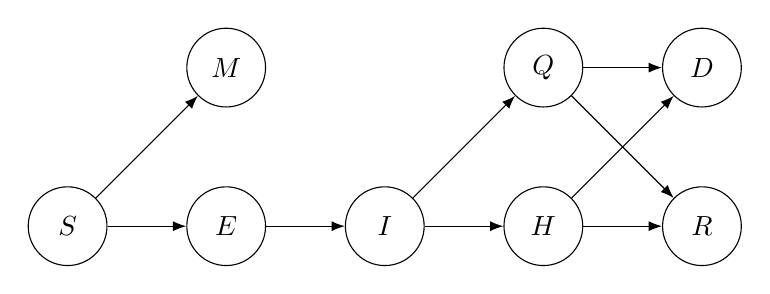
\begin{tikzpicture}[node distance=1cm, auto,
    >=Latex, 
    every node/.append style={align=center},
    int/.style={draw, minimum size=1cm, circle}]
   \node [int] (S)             {$S$};
   \node [int, right=of S] (E) {$E$};
   \node [int, right=of E] (I) {$I$};
   \node [int, right=of I] (H) {$H$};
   \node [int, above=of H] (Q) {$Q$};
   \node [int, right=of Q] (D) {$D$};
   \node [int, right=of H] (R) {$R$};
   \node [int, above=of E] (M) {$M$};

   \path[->] (S) edge node {} (E)
   (E) edge node {} (I)
   (I) edge node {} (H)
   (I) edge node {} (Q)
   (Q) edge node {} (D)
   (Q) edge node {} (R)
   (H) edge node {} (D)
   (H) edge node {} (R)
   (S) edge node {} (M);
\end{tikzpicture}
    \caption{The states for an area $a$}
    \label{fig:SEIR}
\end{figure}
\textbf{Parameters}\\
Each rate is in units of proportion per day.\\
\begin{tabular}{rl}
$r^d$ &rate of detection, either from a self-diagnosis or from a positive test.\\ % set to $\frac{ln(2)}{2}$\\
$p^d$ &Proportion of true cases detected. Some are undetected due to limited testing,\\ &asymptomatic carriers, and detection errors.\\ %, set at 0.2.\\
$p^H$ &Proportion of detected people who need hospitalization.\\ %, set at 0.03 \\
$r^R$ &the rate of recovery or death out of states Q and H. \\
$\beta$ & Vaccine effectiveness. Proportion who become immune via vaccine\\
$A$ &The set of areas.\\
$T_D$  &Time for a variant to dominate (days).\\
$m_a$ &Constant mortality rate in each area.\\
$N_a$ &Initial population in area $a$.\\
$\lambda$ & Increase to infection rate of next variant due to mutation. Unitless.\\
$T$ &Length of time horizon for model (days).\\
$N$ &Number of infected person-days, globally, between variants.\\
$t_N$ &Day when global infection-days exceeds $N$. \\
& Defined as the first day where $\displaystyle \sum_{a=1}^{|A|} \int_0^{t_N} I_a(t) dt \geq N$\\
$p$ &proportion of people in state I that have the new variant when it is introduced in an area.
\end{tabular}\\
\begin{tabular}{rl}
$S_a(0),$ $E_a(0), I_a(0)$ &initial population in a state
\end{tabular}
\section{Other Variables}
\begin{tabular}{rl}
    $V_a(t)$ &The number of people vaccinated per day in each area $a$ at time $t$. A decision variable.\\
    $\alpha_a(t)$ &The infection rate in area $a$ at time $t$.\\
    $\gamma_a(t)$ & Governmental and societal response (unitless). Measures reduction of virus transmission.
\end{tabular}




\section{SEIR Model}
The SEIR model describes the movement of individuals through states. In this section, there are separate dynamics for each area $a$ (region of the world). There are no age groups or risk groups. Areas interact through variants, which occur based on global infections. The Appendix \ref{appendix:travel} adds inter-area travel.\\
\section{Model Assumptions}
    \subsection{Vaccination} A proportion $\beta$ of vaccinated individuals become immediately, permanently immune to the virus. This makes $M$ a terminal state. See Appendix \ref{appendix:VPE} for a version of vaccination that accounts for partial immunity.
        
     \subsection{Infection}  People in state $I$ stay infectious until something causes them to leave. We call this process "detection" even though there are a few ways to stop being infectious. If an infectious person gets a positive test and shows severe symptoms, they get hospitalized and enter state $H$ with proability $p^H$. Otherwise, they go into state $Q$. This state $Q$ is meant to hold those who self-quarantine after self-diagnosis or a positive test. However, the state also holds asymptomatic individuals and those who refuse to self-quarantine. Our model doesn't allow them to still infect others.\\
     There are two reasons for this. The first reason is that it's hard to estimate the number of people in these categories.\\
     The second reason is that asymptomatic infections are rare. A recent meta-analysis by Byambasuren et. al \cite{Byam} estimated that 17\% of disease carries are asymptomatic, and that these carriers are 42\% less likely to transmit the virus than a symptomatic carrier.
     
     %who should  We assume that time until detection is a random variable with an exponential distribution. The mean time until detection is 2 days (Wang Et al. Citation needed,) so the parameter $\lambda$ for the exponential is 0.5.\\
     %At the right tail of the distribution we have individuals who remain infectious for a long time. These individuals are those who initially refuse to self-quarantine or hospitalize.\\
     %We say people leave state $I$ as rate $r^d = \frac{ln(2)}{2}$, the median of an exponential with parameter $\lambda = 2$ that represents detection.
     
     %When people leave state $I$, they cease to infect others. This can happen in a few ways. They can become hospitalized (going to state H) or they could self quarantine (going to state Q.) They go to state H if they need hospitalization (probability $p^H$) and they also are detected with a positive test with probability $p^d$. Otherwise, they self-quarantine after noticing symptoms or after testing positive. 
     %They either become hospitalized or they self-quarantine.
     %as they are detected.
     %We assume that time until detection is a random variable with an exponential distribution. The mean time until detection is 2 days (Wang Et al. Citation needed.) We say they leave detection after the median time of detection,$ \frac{ln(2)}{2. }$.
     %Detection is a Once they leave they no longer infect others. They become hospitalized with rate $p^Hp^d$, the probability they're both discovered and need hospitalization. 

\subsection{Reproduction rate and Mutation}
In Schwarzendahl et al., \cite{m2}, the inherent reproduction rate of the virus increases continuously, either linearly over time or in proportion to the current number of people infected. Instead, we propose that the reproduction rate $\alpha_a(t)$ increases by $\lambda$ after each variant appears. We assume that a variant appears once the global number of person-days infected reaches $N$. Thus, we are assuming that each person in state $I$ contributes the same mutation risk (per day) and are assuming $N$ is deterministic. 

For a given SEIR model, $N$ occurs at some time $t_N$. We assume that the mutation occurs in the area with the largest number of infected person-days, which we call area 1. In this area the variant becomes dominant after a delay of $T$ days and the mixture of the two variants changes over time according to
\begin{equation}\label{eq:infection_rate}
        \alpha_{1}(t) = a_0 + \frac{a_1 - a_0}{1+e^{-k(t-(t_N + T_D))}}
    \end{equation}
Here $k=ln\left(\frac{1-p}{p}\right)/T$, so that $a_1(t_N) = a_0 + (a_1-a_0)p$, i.e. $p$ is the proportion of the new variant at time $t_N$.
    
    
    To visualize, see this temporary graphic:\\
    \begin{figure}[!ht]
        \centering
        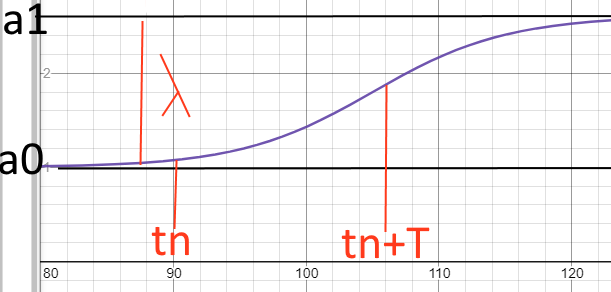
\includegraphics[scale=.5]{alpha equation 2.png}
        \caption{The infection rate $\alpha(t)$ going through a mutation with parameters $t_N = 90, T_D=15, k=0.2, \lambda = 1.6$}
        \label{fig:mutation}
    \end{figure}
    Multiple variants should be able to occur. To be consistent with the linear (increasing) model in \cite{m2}, more variants would occur, separated by $N$ people-days of infection. These variants spread to other areas with aa lag $L$, so that \begin{equation}
        \alpha_a(t) = \alpha_1(t+L) \text{   for }a \neq 1\text{}.\end{equation}\\
    \subsection{Governmental and societal response} We use a unitless rate $\gamma_a(t)$ as multiplier due to governmental and societal response, which varies with cases and then approaches a new normal.\\
    Governmental and societal response is modeled as something like:
    \begin{figure}[!ht]
        \centering
        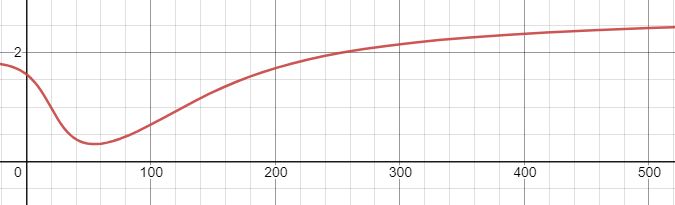
\includegraphics[scale=.6]{gamma.png}
        \caption{$\gamma(t)$ with $k=20$}
        \label{fig:gamma}
    \end{figure}\\
        \begin{equation}
        \gamma(t)_a = -\text{arctan}\left(\frac{t}{k}-1\right)+1.5\text{ arctan}\left(\frac{t}{100}-1\right)+2
    \end{equation}
    where $k$ is the strength of the governmental/societal response, and 1.5 and 100 control the return to \say{new normal.}\\
    \subsection{Mortality rate} 
    The Johns Hopkins University Center for Systems Science and Engineering has \href{https://ourworldindata.org/mortality-risk-covid}{kept track of} COVID-19 mortality rates. Since the start of the pandemic, the mortality rate has decreased over time in all areas. After the first wave of the virus, the mortality rate in each area plateaud. It did not change much when the delta variant took over. It declined recently due to a younger average age and due to effective drugs that have been approved for treatment. We model mortality rate in area $a$ by a constant $m_{a}$.
    \subsection{Vital Dynamics} We omit vital dynamics (birth and death) as a simplifying assumption.     Instead, the sum of all people over all the SEIR states is held constant, even as the death state accumulates. See the appendix for how Vital Dynamics could be implemented.

   

%\begin{table}[!ht]
    %\centering
    %\begin{tabular}{|c|c|c|c|}
    %\hline
        %Parameter & Description & Value & Where found \\
        %\hline
        %$p_h$ & Hospitalization Percentage & .03 & meta-analysis \\
        %\hline
        %RecoverHD & Average Days until Recovery & 15 & meta-analysis \\
        %\hline
        %VentilationD & Recovery time on Ventilation & 10 & meta-analysis \\
        %\hline
        %$p_d$ & Percentage of True Cases Detected & .2 & meta-analysis \\
        %\hline
        %$p_v$ & Percentage of Hospitalized Patients Ventilated, & .25 & meta-analysis \\
        %\hline
        %balance & Regularization coefficient between cases and deaths & & meta-analysis \\
        %\hline
        %$r_i$ & rate of infection leaving incubation &$ \frac{ln(2)}{5}$ &\\
        %\hline
        %$r_d $& rate of detection &$\frac{ln(2)}{2}$ &\\
        %\hline
        %$r_{ri}$ & rate of recovery not under infection &$\frac{ln(2)}{10} $&\\
        %\hline
        %$r_rh$ & rate of recovery under hospitalization & $\frac{ln(2)}{15}$ &\\
        %\hline
        %$r_rv$ & rate of recovery under vent &$\frac{ln(2)}{10}$ &\\
        %\hline
%         
    %\end{tabular}
    %\caption{Some parameters}
    %\label{tab:my_label}
%\end{table}








%\begin{figure}[!ht]
%    \centering
%    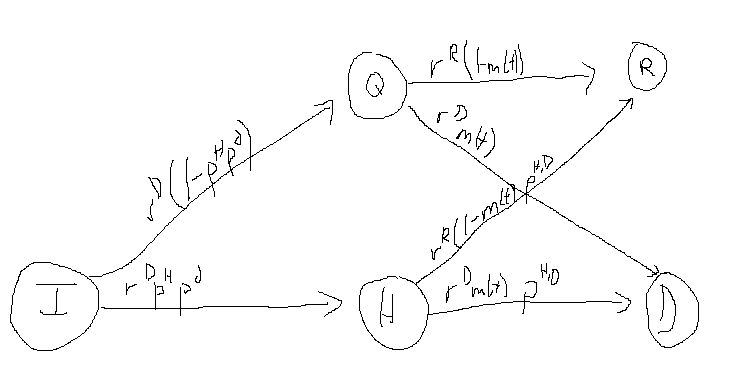
\includegraphics[scale=.7]{from I onward graphic.png}
%    \caption{Rates from I to Q,H and to R,D}
%\end{figure}







\subsection{SEIR Model Equations}
\begin{align}
    \frac{\text{d}S_a}{\text{d}t}&=  -\beta V_a(t) - \alpha_a(t) \gamma_a(t)\frac{S_a(t)}{N_a}I_a(t) \label{eq:S}\\
     \frac{\text{d}E_a}{\text{d}t} &= \alpha_a(t) \gamma_a(t)\frac{S_a(t)}{N_a}I_a(t) -r^IE_a(t) \label{eq:E} \\
     \frac{\text{d}I_a}{\text{d}t}&= r^IE_a(t) - r^dI_a(t)\\
    \frac{\text{d}Q_a}{\text{d}t} &= r^d(1-p^H)I_a(t) - r^RQ_a(t) \\
    \frac{\text{d}H_a}{\text{d}t} &= r^dp^HI_a(t) - r^RH_a(t)\\
    \frac{\text{d}D_a}{\text{d}t} &= r^Rm_a\Big[Q_a(t)+H_a(t)\Big]\\
    \frac{\text{d}R_a}{\text{d}t} &= r^R(1-m_a)\Big[Q_a(t)+H_a(t))\Big]\\
    \frac{\text{d}M_a}{\text{d}t} &= \beta V_a(t) \label{eq:M}
    %\frac{\text{d}\alpha_a}{\text{d}t} &= r^a\frac{\sum_{l=1}^{\mid A \mid}\alpha_l(t)T_{l,a}}{\sum_{l=1}^{\mid A \mid}T_{l,a}}-r^a\alpha_a(t)+\lambda I_a(t)
\end{align}

\subsection{Future Work}
The model could be adjusted to reflect the spread of the virus by asymptomatic individuals.




\section{Vaccine optimization model}
We formulate an optimization model to find the vaccine allocation to minimize deaths over a time horizon. %Define the additional parameters: \\
\textbf{Parameters:}\\
\begin{tabular}{rl}
$B(t) $ &total vaccine doses available in time $t$\\
$\rho_a$ &proportion willing to be vaccinated in area $a$\\
$\delta_a$ &maximum that the fraction vaccinated per day in an area $a$ can change per day\\
$f_a^{max}$ &maximum fraction that can be vaccinated per day, per area $a$.    \\
$T$ &Time Horizon
\end{tabular}\\







For the optimization problem, we use a discrete-time version of the SEIR dynamics with a time step of one day. The difference equations are, e.g., 
\begin{equation}
    M_a(t+1) = M_a(t) + \beta V_a(t)
\end{equation}
The optimization model is
\begin{equation*}
\begin{array}{rlllr}
    \text{min     }  \displaystyle \sum_{a=1}^{|A|}D_a(T) &  & &  & \text{(Deaths in time horizon)}\\
    \text{s.t.    } \displaystyle \sum_{a=1}^{|A|}V_a(t)& \leq B_t  &t = 0,\cdots, T-1 &  &\text{(Vaccination budget)} \\
    M_a(t) &\leq \rho_a S_a(0)  & t = 0,\cdots, T-1,& a \in A &\text{(Vaccine willingness)}\\
    V_a(t) &\leq f_a^{max}S_a(0)  & t = 0,\cdots, T-1,& a \in A &\text{(Vaccine capacity)} \\
    |(V_a(t+1)-V_a(t))| &\leq \delta_aS_a(0)  & t = 0,\cdots, T-1,& a \in A &\text{(Vaccine agility)} \\
    S_a(t+1) &\geq S_a(t)  -\beta V_a(t) - \alpha_a(t) \gamma_a(t)\frac{S_a(t)}{N_a}I_a(t) & t = 0,\cdots, T-1,& a \in A\\
    E_a(t+1) &\geq E_a(t) + \alpha_a(t) \gamma_a(t)\frac{S_a(t)}{N_a}I_a(t) -r^IE_a(t)  & t = 0,\cdots, T-1,& a \in A\\
    I_a(t+1) &\geq I_a(t) + r^IE_a(t) - r^dI_a(t) & t = 0,\cdots, T-1,& a \in A\\
    Q_a(t+1) &\geq Q_a(t) + r^d(1-p^dp^H)I_a(t) - r^RQ_a(t)  & t = 0,\cdots, T-1,& a \in A\\
    H_a(t+1) &\geq H_a(t) + r^dp^Hp^dI_a(t) - r^RH_a(t) & t = 0,\cdots, T-1,& a \in A\\
    D_a(t+1) &= D_a(t) + r^Rm_a\Big[Q_a(t)+H_a(t)\Big] & t = 0,\cdots, T-1,& a \in A\\
    R_a(t+1) &= R_a(t) + r^R(1-m_a)\Big[Q_a(t)+H_a(t))\Big] & t = 0,\cdots, T-1,& a \in A\\
    M_a(t+1) &= M_a(t) +\beta V_a(t)  & t = 0,\cdots, T-1,& a \in A\\
    \multicolumn{2}{l}{S_a(t), E_a(t), I_a(t), Q_a(t), H_a(t), V_a(t) \geq 0 } & t = 0,\cdots, T-1,& a \in A &\text{(Nonnegativity)}
\end{array}
\end{equation*}


Although the constraints are nonlinear, an iterative process can be used to solve this optimization problem as in  (Bertsimas, et. al, 2021) \cite{a1}. In each iteration, given the current solution $V$, solve the difference equations to get $\hat{I}_a(t)$. In the (nonlinear) constraints for $S$ and $E$, replace the variables $I$ with the constants $\hat{I}$ . Omit the constraints for $I$ and add the regularization constraints
\begin{equation}
\begin{array}{clrr}
    \mid I_a(t) - \hat{I}_a(t) \mid \leq \epsilon & & t = 0, \cdots, T-1, & a \in A
    \end{array}
\end{equation}
Here, $\epsilon > 0$ is an error tolerance. This linear program can be solved to find the best solution $V^*$ that gives infection dynamics $I$ that are close to $\hat{I}$ , i.e., close to those of the current solution. The current solution $V$ is updated and the process repeated until the objective function value converges. Other stopping criteria could also be used, as in \cite{a1}.

\section{Uses of the model}
This model is meant to describe COVID-19 on a global scale. One application would be to imagine four areas, as shown in table \ref{tab:four-areas}.\\

\begin{table}
\centering
    \setlength{\extrarowheight}{2pt}
    \begin{tabular}{cc|c|c|}
      & \multicolumn{1}{c}{} & \multicolumn{2}{c}{Vaccinations}\\
      & \multicolumn{1}{c}{} & \multicolumn{1}{c}{High}  & \multicolumn{1}{c}{Low} \\\cline{3-4}
      \multirow{2}*{Travel}  & High & Area 1 & Area 2 \\\cline{3-4}
      & Low & Area 3 & Area 4 \\\cline{3-4}
    \end{tabular}
    \caption{The four areas, defined by vaccination and travel rates.}
\label{tab:four-areas}
  \end{table}
Here are some of the countries in each area. It's a work in progress, as the destinction between the areas is blurred. Data and code is documented in the  \href{https://github.com/Stonepaw90/international-vaccine-allocation}{International Vaccine Allocation gitHhb}.

\begin{table}[!ht]
    \centering
    \begin{tabular}{|c|c|c|c|c|}
    \hline
         area & Country & $\frac{\text{total vaccinations}}{\text{population}}$\%  & $\frac{\text{total passengers}}{\text{population}}$ & population \\
         \hline
1 & Canada & 80.79 & 2.45 & 38,067,913 \\
1 & Ireland & 77.5 & 34.14 & 4,982,904 \\
1 & Japan & 79.22 & 1.03 & 126,050,796 \\
1 & United Arab Emirates & 98.10  & 9.2 & 9,991,083 \\
1 & United Kingdom& 74.87 & 2.08 & 682,071,14  \\
1 & United States & 70.87 & 2.78 & 332,915,074 \\
\hline
2 & Bahamas & 38.2 & 4.67 & 396,914 \\
2 & India & 57.39 & 0.12  & 1,393,409,033 \\
2 & Indonesia & 51.54 & 0.33  & 276,361,788 \\
2 & Mexico & 59.39 & 0.53  & 130,262,220 \\
2 & Russia & 46.60 & 0.79  & 145,912,022 \\
2 & South Africa & 29.41 & 0.42  & 60,041,996 \\
\hline
3 & Argentina & 81.07 & 0.42  & 45,605,823 \\
3 & Cambodia & 83.55 & 0.08 8 & 16,946,446 \\
3 & Colombia & 74.41 & 0.72  & 51,265,841 \\
3 & Cuba & 90.02 & 0.040 & 11,317,498 \\
3 & Ecuador & 77.12 & 0.26  & 17,888,474 \\
3 & Iran & 67.49 & 0.25  & 85,028,760 \\
\hline
4 & Ethiopia & 7.06 & 0.10  & 117,876,226 \\
4 & Ghana & 8.36 & 0.019 & 31,732,128 \\
4 & Kenya & 8.9 & 0.117  & 54,985,702 \\
4 & Mozambique & 20.4 & 0.018 & 32,163,045 \\
4 & Nigeria & 3.09 & 0.031 & 211,400,704 \\
4 & Uganda & 8.15 & 0.0004 & 47,123,533 \\
\hline


    \end{tabular}
    \caption{Vaccination rates and flights per person for each country in each area}
    \label{tab:vax}
\end{table}
In this case, it would be useful to include the vaccine partial effectiveness assumption from \ref{appendix:VPE}. That way, vaccination prevents more people from contributing to mutation. 
%A1: 1 13 19 28 38 14
%A2: 84 106 68 66 75 96
%a3: 4 7 20 30 12 54
%a4: 118, 130, 131, 132, 135, 139


The interactions between these areas could shed insight on the effectiveness of vaccines to reduce mutations. That is, how beneficial is a vaccine when it is used on area 2?
tic or  movement of asymtomatic
\newpage
\bibliographystyle{ieeetr}
%\bibliographystyle{IEEEtran}
%\bibliography{IEEEabrv, references}
\bibliography{references}


































\newpage
\section{Appendix: Model additions}

\subsection{Inter-area Travel}\label{appendix:travel}

This addition accounts for the spread of the virus from travelling between areas. Infected travelers expose those in their area of destination. \\
\textbf{Parameters}:\\
\begin{tabular}{rl}
$T_{a,l}$ & Number of passengers on flights from area $a$ to area $l$ per year.\\% For example, \\&if 100 million passengers left Canada, and 30 million went to America,\\&then $p_{Canada, USA} = 0.3$.\\
%$P_a$ & Number of passengers leaving area $a$, or $\displaystyle \sum_{l=1}^{|A|}T_{a,l}$.\\
\end{tabular}\\
The median infectious person stays undetected for $\frac{ln(2)}{r^d}$ days, so that's their duration of infectiousness. 
The number of people from area $a$ who are in area $l$ who are also infectious is $\frac{T_{a,l}}{365}\frac{I_a(t)}{N_a}\frac{ln(2)}{r^d}$. It's the number of travellers from $a$ to $l$ per day, times the proportion of those who are infectious, times their duration of infectiousness.\\
With this addition, the SEIR equations (\ref{eq:S}) and (\ref{eq:E}) become:
\begin{equation}
    \frac{\text{d}S_a}{\text{d}t}= -\beta V_a(t) - \alpha_a(t) \gamma_a(t)\frac{S_a(t)}{N_a}\left(I_a(t) +  \sum\limits_{l=1}^{|A|} \frac{T_{l,a}}{365}\frac{I_l}{N_l}\frac{ln(2)}{r^d} -   \sum\limits_{a=1}^{|A|} \frac{T_{a,l}}{365}\frac{I_a}{N_a}\frac{ln(2)}{r^d}     \right)
\end{equation}
\begin{equation}
        \frac{\text{d}E_a}{\text{d}t} = \alpha_a(t) \gamma_a(t)\frac{S_a(t)}{N_a}\left(I_a(t) +  \sum\limits_{l=1}^{|A|} \frac{T_{l,a}}{365}\frac{I_l}{N_l}\frac{ln(2)}{r^d} -   \sum\limits_{a=1}^{|A|} \frac{T_{a,l}}{365}\frac{I_a}{N_a}\frac{ln(2)}{r^d}    \right) -r^IE_a(t)
\end{equation}
The term $I_a(t) +  \sum\limits_{l=1}^{|A|} \frac{T_{l,a}}{365}\frac{I_l}{N_l}\frac{ln(2)}{r^d} -   \sum\limits_{a=1}^{|A|} \frac{T_{a,l}}{365}\frac{I_a}{N_a}\frac{ln(2)}{r^d}$ represents the people infected, plus the out of country infectious people in $a$, less the infectious people from $a$ who are in other areas.\\
The SEIR equations (\ref{eq:S})-(\ref{eq:M}) for the other states are unchanged.



%The way I implemented travel was inadvertently causing the populations of different areas to slowly blend together. Each area was becoming like those areas around it. This would only be the case if travellers stayed in their country of destination. Really, travelers come, infect a few people, and then come back. In reality, there is no blending of different areas.
%What about infection due to travel? When an infected person takes a plane into another area, they infect the people in their area of destination. However, they are no different at infecting others than a native of that area. So, when an infected native leaves, the effects cancel out: one has entered, one has left.
%Once we've canceled out these people, we're left with a net positive number of infected people temporarily entering an area. They arrive, infect, and then notice symptoms. If they recover, they travel back. When all is said and done, they have exposed a few people in their area of destination and they have prevented people from being exposed in their home area. (And they have added deaths in their area of destination.) Hence, travel merely contributes a marginal change to the number of exposed people. This is a second-order effect.
%What about the infection rate? Yes, international travel is the only way to for $\alpha_{max}$ to spread. Hence, travel is best used to modify the spread of variants. 

\subsection{Vital Dynamics}
Vital dynamics (births and non-pandemic related deaths) are significant when simulating a long time horizon. \\
\textbf{Parameters:}\\
\begin{tabular}{rl}
$\mu$ &Death rate (proportion of population per day)\\
\end{tabular}\\
We make the simplifying assumption that the number of births equals the number of natural deaths. We add the births, $\mu N_a$, into the susceptible state. Deaths leave all other states except $D$, e.g. $-\mu S_a(t)$ for state $S_a$.\\
A simplified diagram shows the addition of vital dynamics. In this simple version, $N_a = S_a + I_a + R_a$.\\
\begin{figure}[!ht]
    \centering
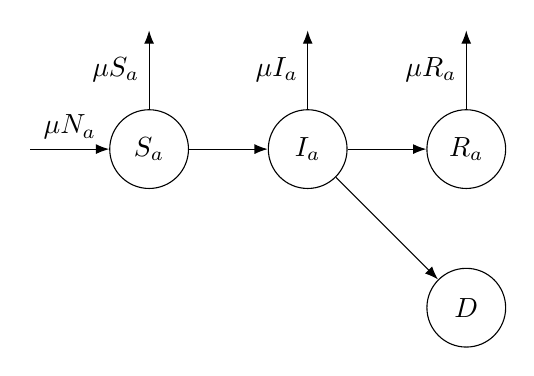
\begin{tikzpicture}[node distance=1cm, auto,
    >=Latex, 
    every node/.append style={align=center},
    int/.style={draw, minimum size=1cm, circle}]
    \tikzstyle{connection}=[inner sep=0,outer sep=0]

    
   \node [int] (S)             {$S_a$};
   \node [int, right=of S] (I) {$I_a$};
   \node [int, right=of I] (R) {$R_a$};
      \node [int, below=of R] (D) {$D$};
    \node [connection, left=of S] (B) {};
    \node [connection, above=of S] (D1) {};
    \node [connection, above=of I] (D2) {};
    \node [connection, above=of R] (D3) {};

   \path[->] (S) edge node {} (I)
   (I) edge node {} (R)
   (I) edge node {} (D)
   (B) edge node {$\mu N_a$} (S)
   (S) edge node {$\mu S_a$} (D1)
   (I) edge node {$\mu I_a$} (D2)
   (R) edge node {$\mu R_a$} (D3);
   %[right=of S] edge node {} (S);
\end{tikzpicture}
    \caption{The dynamics of births and deaths on a simple SIR model}
    \label{fig:SEIR-V}
\end{figure}

The full model, with vital dynamics, would be:\\
\begin{align}
    \frac{\text{d}S_a}{\text{d}t}&=  -\beta V_a(t) - \alpha_a(t) \gamma_a(t)\frac{S_a(t)}{N_a}I_a(t) + \mu N_a - \mu S_a \label{eq:start-vital}\\
     \frac{\text{d}E_a}{\text{d}t} &= \alpha_a(t) \gamma_a(t)\frac{S_a(t)}{N_a}I_a(t) -r^IE_a(t) - \mu E_a \\
     \frac{\text{d}I_a}{\text{d}t}&= r^IE_a(t) - r^dI_a(t)- \mu I_a\\
    \frac{\text{d}Q_a}{\text{d}t} &= r^d(1-p^dp^H)I_a(t) - r^RQ_a(t) - \mu Q_a \\
    \frac{\text{d}H_a}{\text{d}t} &= r^dp^Hp^dI_a(t) - r^RH_a(t) - \mu H_a\\
    \frac{\text{d}D_a}{\text{d}t} &= r^Rm_a\Big[Q_a(t)+H_a(t)\Big]\\
    \frac{\text{d}R_a}{\text{d}t} &= r^R(1-m_a)\Big[Q_a(t)+H_a(t))\Big] - \mu R_a\\
    \frac{\text{d}M_a}{\text{d}t} &= \beta V_a(t) - \mu M_a \label{eq:end-vital}
    %\frac{\text{d}\alpha_a}{\text{d}t} &= r^a\frac{\sum_{l=1}^{\mid A \mid}\alpha_l(t)T_{l,a}}{\sum_{l=1}^{\mid A \mid}T_{l,a}}-r^a\alpha_a(t)+\lambda I_a(t)
\end{align}


\subsection{Vaccine Partial effectiveness}\label{appendix:VPE}
It is more realistic for the vaccine to give people partial immunity rather than giving a proportion of people full immunity. Here, everyone who is vaccinated at time $t$ in area $a$, $V_a(t)$, is brought into a new set of states.\\
\textbf{State Variables:}\\
\begin{tabular}{rl}
$S^V_a$ &Susceptible and vaccinated\\
$E^V_a$ &Exposed and vaccinated\\
$I^V_a$ &Infectious and vaccinated\\
\end{tabular}\\
These states are added to figure \ref{fig:SEIR}.
\begin{figure}[!ht]
    \centering
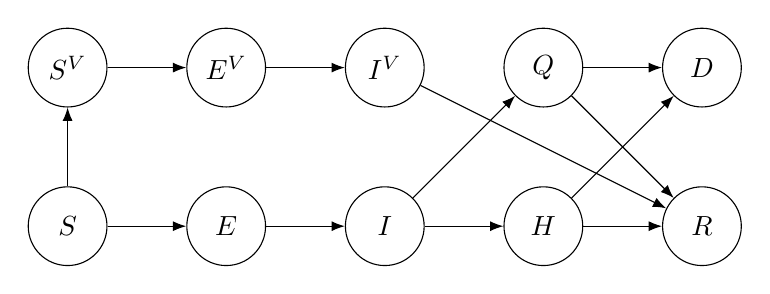
\begin{tikzpicture}[node distance=1cm, auto,
    >=Latex, 
    every node/.append style={align=center},
    int/.style={draw, minimum size=1cm, circle}]
   \node [int] (S)             {$S$};
   \node [int, right=of S] (E) {$E$};
   \node [int, right=of E] (I) {$I$};
   \node [int, right=of I] (H) {$H$};
   \node [int, above=of H] (Q) {$Q$};
   \node [int, right=of Q] (D) {$D$};
   \node [int, right=of H] (R) {$R$};
  % \node [int, above=of E] (M) {$M$};
    
    \node [int, above=of S] (SV) {$S^V$};
    \node [int, above=of E] (EV) {$E^V$};
    \node [int, above=of I] (IV) {$I^V$};


   \path[->] (S) edge node {} (E)
   (E) edge node {} (I)
   (I) edge node {} (H)
   (I) edge node {} (Q)
   (Q) edge node {} (D)
   (Q) edge node {} (R)
   (H) edge node {} (D)
   (H) edge node {} (R)
   %(S) edge node {} (M)
   (S) edge node {} (SV)
   (SV) edge node {} (EV)
   (EV) edge node {} (IV)
   (IV) edge node {} (R);
\end{tikzpicture}
    \caption{The states for an area $a$ with a vaccination track}
    \label{fig:SEIR-V}
\end{figure}

\textbf{Parameters:}\\
\begin{tabular}{rl}
$p^e$ &Vaccine effectiveness at reducing transmission\\
$p^r$ &Vaccine protection against receiving the virus
\end{tabular}\\

As you can see in Figure \ref{fig:SEIR-V}, those who are vaccinated can get sick but they can't die. This assumption is due to the observed reduced mortality of breakthrough cases. The population $I^V$ is less infectious than the state $I$ due to the vaccine's effectiveness against transmission: an infectious person who has been vaccinated is only $1-p^e$ as infectious as an unvaccinated individual. Those who are vaccinated are less likely to receive the virus. We represent this with the proportion $p^r$.\\
%(inspired by https://www.medrxiv.org/content/medrxiv/suppl/2020/03/06/2020.03.03.20030593.DC1/2020.03.03.20030593-1.pdf)
\\
\subsection{SEIR Model with vaccination}
\begin{align}
    \frac{\text{d}S_a}{\text{d}t}&=  -V_a(t) - \alpha_a(t) \gamma_a(t)\frac{S_a(t)}{N_a}\big[I_a(t)+(1-p^e)I^V_a(t)\big] \label{eq:start-SEIRV}\\
     \frac{\text{d}E_a}{\text{d}t} &= \alpha_a(t) \gamma_a(t)\frac{S_a(t)}{N_a}\big[I_a(t)+(1-p^e)I^V_a(t)\big] -r^IE_a(t) \\
     \frac{\text{d}I_a}{\text{d}t}&= r^IE_a(t) - r^dI_a(t)\\
    \frac{\text{d}S^V_a}{\text{d}t}&=  V_a(t) - p^r\alpha_a(t) \gamma_a(t)\frac{S^V_a(t)}{N_a}\big[I_a(t)+(1-p^e)I^V_a(t)\big]\\
     \frac{\text{d}E^V_a}{\text{d}t} &= p^r \alpha_a(t) \gamma_a(t)\frac{S^V_a(t)}{N_a}\big[I_a(t)+(1-p^e)I^V_a(t)\big] -r^IE^V_a(t) \\
     \frac{\text{d}I^V_a}{\text{d}t}&= r^IE^V_a(t) - r^dI^V_a(t)\\   
    \frac{\text{d}Q_a}{\text{d}t} &= r^d(1-p^dp^H)I_a(t) - r^RQ_a(t) \\
    \frac{\text{d}H_a}{\text{d}t} &= r^dp^Hp^dI_a(t) - r^RH_a(t)\\
    \frac{\text{d}D_a}{\text{d}t} &= r^Rm_a\Big[Q_a(t)+H_a(t)\Big]\\
    \frac{\text{d}R_a}{\text{d}t} &= r^R(1-m_a)\Big[Q_a(t)+H_a(t))\Big] \label{eq:end-SEIRV}
    %\frac{\text{d}\alpha_a}{\text{d}t} &= r^a\frac{\sum_{l=1}^{\mid A \mid}\alpha_l(t)T_{l,a}}{\sum_{l=1}^{\mid A \mid}T_{l,a}}-r^a\alpha_a(t)+\lambda I_a(t)
\end{align}
We assume that breakthrough cases do not contribute to mutation because the cirus replicates less. Hence, $t_N$ is computed from $I$, not $I^V$.
\end{document}